\documentclass[a4paper]{article}\usepackage[]{graphicx}\usepackage[]{color}
%% maxwidth is the original width if it is less than linewidth
%% otherwise use linewidth (to make sure the graphics do not exceed the margin)
\makeatletter
\def\maxwidth{ %
  \ifdim\Gin@nat@width>\linewidth
    \linewidth
  \else
    \Gin@nat@width
  \fi
}
\makeatother

\definecolor{fgcolor}{rgb}{0.345, 0.345, 0.345}
\newcommand{\hlnum}[1]{\textcolor[rgb]{0.686,0.059,0.569}{#1}}%
\newcommand{\hlstr}[1]{\textcolor[rgb]{0.192,0.494,0.8}{#1}}%
\newcommand{\hlcom}[1]{\textcolor[rgb]{0.678,0.584,0.686}{\textit{#1}}}%
\newcommand{\hlopt}[1]{\textcolor[rgb]{0,0,0}{#1}}%
\newcommand{\hlstd}[1]{\textcolor[rgb]{0.345,0.345,0.345}{#1}}%
\newcommand{\hlkwa}[1]{\textcolor[rgb]{0.161,0.373,0.58}{\textbf{#1}}}%
\newcommand{\hlkwb}[1]{\textcolor[rgb]{0.69,0.353,0.396}{#1}}%
\newcommand{\hlkwc}[1]{\textcolor[rgb]{0.333,0.667,0.333}{#1}}%
\newcommand{\hlkwd}[1]{\textcolor[rgb]{0.737,0.353,0.396}{\textbf{#1}}}%

\usepackage{framed}
\makeatletter
\newenvironment{kframe}{%
 \def\at@end@of@kframe{}%
 \ifinner\ifhmode%
  \def\at@end@of@kframe{\end{minipage}}%
  \begin{minipage}{\columnwidth}%
 \fi\fi%
 \def\FrameCommand##1{\hskip\@totalleftmargin \hskip-\fboxsep
 \colorbox{shadecolor}{##1}\hskip-\fboxsep
     % There is no \\@totalrightmargin, so:
     \hskip-\linewidth \hskip-\@totalleftmargin \hskip\columnwidth}%
 \MakeFramed {\advance\hsize-\width
   \@totalleftmargin\z@ \linewidth\hsize
   \@setminipage}}%
 {\par\unskip\endMakeFramed%
 \at@end@of@kframe}
\makeatother

\definecolor{shadecolor}{rgb}{.97, .97, .97}
\definecolor{messagecolor}{rgb}{0, 0, 0}
\definecolor{warningcolor}{rgb}{1, 0, 1}
\definecolor{errorcolor}{rgb}{1, 0, 0}
\newenvironment{knitrout}{}{} % an empty environment to be redefined in TeX

\usepackage{alltt}
\usepackage[british]{babel}
\usepackage{booktabs}
\IfFileExists{upquote.sty}{\usepackage{upquote}}{}
\begin{document}

\title{A Preprocessing Pipeline for Exposome Data}
\author{Jeff Sorbo}
\maketitle\thispagestyle{empty}

\section{Introduction}

This project will include multiple preprocessing techniques for exposome data.

\section{Business Problem}

Describe discussions with client (business experts) and record
decisions made and shared understanding of the business problem.

\section{Data Sources}

Identify the data sources and discuss access with the data
owners. Document data sources, integrity, providence, and dates.

\section{Data Preparation}

Load the data into R and perform various operations on the data to
shape it for modelling.

\section{Data Exploration}

We should always understand our data by exploring it in various
ways. Include data summaries and various plots that give insights.

\section{Model Building}

Include all models built and parameters tried. Include R code and
model evaluations.

\section{Deployment}

Choose the model to deploy and export it, perhaps as PMML.

\section{Echoing Code}

\begin{knitrout}
\definecolor{shadecolor}{rgb}{0.969, 0.969, 0.969}\color{fgcolor}\begin{kframe}
\begin{alltt}
\hlstd{x} \hlkwb{<-} \hlkwd{runif}\hlstd{(}\hlnum{1000}\hlstd{)} \hlopt{*} \hlnum{1000}
\hlkwd{head}\hlstd{(x)}
\end{alltt}
\begin{verbatim}
## [1] 591.14071 102.23089 547.29147  23.40307 627.79111 332.79199
\end{verbatim}
\begin{alltt}
\hlkwd{mean}\hlstd{(x)}
\end{alltt}
\begin{verbatim}
## [1] 504.001
\end{verbatim}
\end{kframe}
\end{knitrout}

\section{Non-Echoing Code}

\begin{knitrout}
\definecolor{shadecolor}{rgb}{0.969, 0.969, 0.969}\color{fgcolor}\begin{kframe}
\begin{verbatim}
## [1] 253.3932 855.8366 215.1099 665.8442 929.3086 674.9027
## [1] 508.6685
\end{verbatim}
\end{kframe}
\end{knitrout}

\section{Inline Code}



Today's date is Monday, 19 December 2016.

The weather dataset from rattle (Williams, 2014) has 366 (i.e., 366) observations including
observations of the following 4 variables: MinTemp, MaxTemp, Rainfall, Evaporation
(i.e., MinTemp, MaxTemp, Rainfall, Evaporation).

\section{Table with kable}

\begin{kframe}
\begin{alltt}
\hlcom{#library(rattle)}
\hlkwd{library}\hlstd{(dplyr)}
\end{alltt}


{\ttfamily\noindent\color{warningcolor}{\#\# Warning: package 'dplyr' was built under R version 3.2.5}}

{\ttfamily\noindent\itshape\color{messagecolor}{\#\# \\\#\# Attaching package: 'dplyr'}}

{\ttfamily\noindent\itshape\color{messagecolor}{\#\# The following objects are masked from 'package:stats':\\\#\# \\\#\#\ \ \ \  filter, lag}}

{\ttfamily\noindent\itshape\color{messagecolor}{\#\# The following objects are masked from 'package:base':\\\#\# \\\#\#\ \ \ \  intersect, setdiff, setequal, union}}\begin{alltt}
\hlkwd{set.seed}\hlstd{(}\hlnum{42}\hlstd{)}

\hlstd{dsname} \hlkwb{<-} \hlstr{"weatherAUS"}
\hlstd{ds} \hlkwb{<-} \hlkwd{tbl_df}\hlstd{(}\hlkwd{get}\hlstd{(dsname))}
\hlstd{nobs} \hlkwb{<-} \hlkwd{nrow}\hlstd{(ds)}
\hlstd{obs} \hlkwb{<-} \hlkwd{sample}\hlstd{(nobs,} \hlnum{20}\hlstd{)}
\hlstd{vars} \hlkwb{<-} \hlnum{2}\hlopt{:}\hlnum{7}
\hlstd{ds} \hlkwb{<-} \hlstd{ds[obs, vars]}
\hlkwd{kable}\hlstd{(ds,} \hlkwc{row.names}\hlstd{=}\hlnum{FALSE}\hlstd{,} \hlkwc{digits}\hlstd{=}\hlnum{0}\hlstd{,} \hlkwc{booktabs}\hlstd{=}\hlnum{TRUE}\hlstd{)}
\end{alltt}
\end{kframe}
\begin{tabular}{lrrrrr}
\toprule
Location & MinTemp & MaxTemp & Rainfall & Evaporation & Sunshine\\
\midrule
Hobart & 14 & 22 & 0 & 6 & 9\\
Launceston & -3 & 11 & 0 & NA & NA\\
Williamtown & 11 & 16 & 32 & NA & NA\\
PerthAirport & 9 & 20 & 1 & 1 & 4\\
GoldCoast & 10 & 21 & 0 & NA & NA\\
\addlinespace
Portland & 5 & 16 & 0 & 3 & 12\\
Woomera & 18 & 34 & 0 & NA & NA\\
NorahHead & 19 & 27 & 0 & NA & NA\\
Townsville & 16 & 30 & 0 & 7 & 11\\
MountGambier & 6 & 20 & 0 & 1 & 6\\
\addlinespace
MelbourneAirport & 5 & 21 & 0 & 4 & 9\\
Nuriootpa & 17 & 31 & 0 & 10 & 13\\
Launceston & 9 & 15 & 0 & NA & NA\\
WaggaWagga & 10 & 31 & 0 & 11 & 14\\
MelbourneAirport & 8 & 20 & 0 & 5 & 6\\
\addlinespace
AliceSprings & 23 & 37 & 0 & 13 & 10\\
Darwin & 18 & 34 & 0 & 6 & 9\\
Newcastle & 7 & 19 & 0 & NA & NA\\
Melbourne & 13 & 20 & 0 & 6 & 6\\
Dartmoor & 10 & 17 & 2 & 7 & 8\\
\bottomrule
\end{tabular}



\section{Table with xtable}

\begin{kframe}
\begin{alltt}
\hlcom{#library(rattle)}
\hlkwd{library}\hlstd{(xtable)}
\end{alltt}


{\ttfamily\noindent\color{warningcolor}{\#\# Warning: package 'xtable' was built under R version 3.2.5}}\begin{alltt}
\hlstd{dst} \hlkwb{<-} \hlstd{weatherAUS[}\hlkwd{sample}\hlstd{(nobs,} \hlnum{20}\hlstd{), vars]}
\hlkwd{xtable}\hlstd{(dst)}
\end{alltt}
\end{kframe}% latex table generated in R 3.2.4 by xtable 1.8-2 package
% Mon Dec 19 23:40:19 2016
\begin{table}[ht]
\centering
\begin{tabular}{rlrrrrr}
  \hline
 & Location & MinTemp & MaxTemp & Rainfall & Evaporation & Sunshine \\ 
  \hline
108592 & Hobart & 12.60 & 20.80 & 0.00 & 2.40 & 5.70 \\ 
  16662 & NorahHead & 14.70 & 19.80 & 0.00 &  &  \\ 
  118783 & Katherine & 15.30 & 34.90 & 0.00 & 7.20 &  \\ 
  113711 & AliceSprings & 4.10 & 23.20 & 0.00 & 4.00 & 4.80 \\ 
  9902 & CoffsHarbour & 17.70 & 27.20 & 0.00 &  &  \\ 
  61765 & Nhil & 5.80 & 19.90 & 0.00 &  &  \\ 
  46869 & Ballarat & 7.30 & 26.10 & 0.00 &  &  \\ 
  108791 & Hobart & 10.60 & 20.40 & 0.00 & 4.00 & 9.30 \\ 
  53686 & MelbourneAirport & 18.30 & 21.80 & 0.00 & 15.20 & 0.50 \\ 
  100413 & Perth & 13.20 & 19.60 & 1.00 & 4.20 & 11.00 \\ 
  88592 & Woomera & 15.10 & 22.60 & 15.40 & 1.80 &  \\ 
  97415 & PearceRAAF & 8.10 & 26.00 & 0.00 &  & 12.90 \\ 
  46615 & Ballarat & 11.80 & 28.00 & 0.00 &  &  \\ 
  82293 & Adelaide & 8.80 & 14.30 & 0.40 &  &  \\ 
  475 & Albury & 16.70 & 31.90 & 0.00 &  &  \\ 
  100037 & Perth & 1.00 & 19.00 & 5.40 & 1.60 & 11.10 \\ 
  881 & Albury & 3.60 & 15.90 & 0.00 &  &  \\ 
  24941 & Richmond & 18.10 & 39.70 & 0.00 &  &  \\ 
  108884 & Hobart & 15.80 & 26.30 & 0.60 & 5.60 & 2.40 \\ 
  73475 & Cairns & 15.80 & 25.00 & 0.00 & 5.40 & 10.60 \\ 
   \hline
\end{tabular}
\end{table}
\begin{kframe}\begin{alltt}
\hlkwd{print}\hlstd{(}\hlkwd{xtable}\hlstd{(ds),} \hlkwc{include.rownames}\hlstd{=}\hlnum{FALSE}\hlstd{)}
\end{alltt}
\end{kframe}% latex table generated in R 3.2.4 by xtable 1.8-2 package
% Mon Dec 19 23:40:19 2016
\begin{table}[ht]
\centering
\begin{tabular}{lrrrrr}
  \hline
Location & MinTemp & MaxTemp & Rainfall & Evaporation & Sunshine \\ 
  \hline
Hobart & 13.60 & 22.40 & 0.00 & 5.60 & 8.70 \\ 
  Launceston & -2.80 & 10.80 & 0.20 &  &  \\ 
  Williamtown & 11.10 & 15.70 & 31.60 &  &  \\ 
  PerthAirport & 9.00 & 20.10 & 0.80 & 1.20 & 4.00 \\ 
  GoldCoast & 9.70 & 21.10 & 0.00 &  &  \\ 
  Portland & 5.00 & 15.80 & 0.00 & 3.20 & 12.50 \\ 
  Woomera & 18.50 & 34.30 & 0.00 &  &  \\ 
  NorahHead & 18.80 & 26.70 & 0.00 &  &  \\ 
  Townsville & 15.80 & 29.70 & 0.00 & 7.00 & 10.70 \\ 
  MountGambier & 6.00 & 20.10 & 0.00 & 1.00 & 6.10 \\ 
  MelbourneAirport & 5.20 & 20.90 & 0.00 & 4.20 & 9.30 \\ 
  Nuriootpa & 17.40 & 31.40 & 0.20 & 9.80 & 13.40 \\ 
  Launceston & 8.80 & 14.60 & 0.00 &  &  \\ 
  WaggaWagga & 9.90 & 30.60 & 0.00 & 10.80 & 13.70 \\ 
  MelbourneAirport & 8.00 & 20.00 & 0.00 & 4.80 & 5.50 \\ 
  AliceSprings & 23.00 & 37.30 & 0.20 & 13.20 & 9.60 \\ 
  Darwin & 18.50 & 33.90 & 0.00 & 6.20 & 8.60 \\ 
  Newcastle & 6.90 & 19.20 & 0.00 &  &  \\ 
  Melbourne & 13.10 & 20.20 & 0.00 & 5.80 & 6.00 \\ 
  Dartmoor & 9.70 & 16.70 & 2.40 & 6.60 & 7.70 \\ 
   \hline
\end{tabular}
\end{table}
\begin{kframe}\begin{alltt}
\hlkwd{print}\hlstd{(}\hlkwd{xtable}\hlstd{(ds,} \hlkwc{digits}\hlstd{=}\hlnum{1}\hlstd{),} \hlkwc{include.rownames}\hlstd{=}\hlnum{FALSE}\hlstd{)}
\end{alltt}
\end{kframe}% latex table generated in R 3.2.4 by xtable 1.8-2 package
% Mon Dec 19 23:40:20 2016
\begin{table}[ht]
\centering
\begin{tabular}{lrrrrr}
  \hline
Location & MinTemp & MaxTemp & Rainfall & Evaporation & Sunshine \\ 
  \hline
Hobart & 13.6 & 22.4 & 0.0 & 5.6 & 8.7 \\ 
  Launceston & -2.8 & 10.8 & 0.2 &  &  \\ 
  Williamtown & 11.1 & 15.7 & 31.6 &  &  \\ 
  PerthAirport & 9.0 & 20.1 & 0.8 & 1.2 & 4.0 \\ 
  GoldCoast & 9.7 & 21.1 & 0.0 &  &  \\ 
  Portland & 5.0 & 15.8 & 0.0 & 3.2 & 12.5 \\ 
  Woomera & 18.5 & 34.3 & 0.0 &  &  \\ 
  NorahHead & 18.8 & 26.7 & 0.0 &  &  \\ 
  Townsville & 15.8 & 29.7 & 0.0 & 7.0 & 10.7 \\ 
  MountGambier & 6.0 & 20.1 & 0.0 & 1.0 & 6.1 \\ 
  MelbourneAirport & 5.2 & 20.9 & 0.0 & 4.2 & 9.3 \\ 
  Nuriootpa & 17.4 & 31.4 & 0.2 & 9.8 & 13.4 \\ 
  Launceston & 8.8 & 14.6 & 0.0 &  &  \\ 
  WaggaWagga & 9.9 & 30.6 & 0.0 & 10.8 & 13.7 \\ 
  MelbourneAirport & 8.0 & 20.0 & 0.0 & 4.8 & 5.5 \\ 
  AliceSprings & 23.0 & 37.3 & 0.2 & 13.2 & 9.6 \\ 
  Darwin & 18.5 & 33.9 & 0.0 & 6.2 & 8.6 \\ 
  Newcastle & 6.9 & 19.2 & 0.0 &  &  \\ 
  Melbourne & 13.1 & 20.2 & 0.0 & 5.8 & 6.0 \\ 
  Dartmoor & 9.7 & 16.7 & 2.4 & 6.6 & 7.7 \\ 
   \hline
\end{tabular}
\end{table}
\begin{kframe}\begin{alltt}
\hlstd{dst} \hlkwb{<-} \hlstd{ds}
\hlstd{dst[}\hlopt{-}\hlnum{1}\hlstd{]} \hlkwb{<-} \hlkwd{sample}\hlstd{(}\hlnum{10000}\hlopt{:}\hlnum{99999}\hlstd{,} \hlkwd{nrow}\hlstd{(dst))} \hlopt{*} \hlstd{dst[}\hlopt{-}\hlnum{1}\hlstd{]}
\hlkwd{print}\hlstd{(}\hlkwd{xtable}\hlstd{(dst,} \hlkwc{digits}\hlstd{=}\hlnum{0}\hlstd{),} \hlkwc{include.rownames}\hlstd{=}\hlnum{FALSE}\hlstd{)}
\end{alltt}
\end{kframe}% latex table generated in R 3.2.4 by xtable 1.8-2 package
% Mon Dec 19 23:40:20 2016
\begin{table}[ht]
\centering
\begin{tabular}{lrrrrr}
  \hline
Location & MinTemp & MaxTemp & Rainfall & Evaporation & Sunshine \\ 
  \hline
Hobart & 600576 & 989184 & 0 & 247296 & 384192 \\ 
  Launceston & -137813 & 531565 & 9844 &  &  \\ 
  Williamtown & 148385 & 209878 & 422429 &  &  \\ 
  PerthAirport & 878535 & 1962062 & 78092 & 117138 & 390460 \\ 
  GoldCoast & 473893 & 1030841 & 0 &  &  \\ 
  Portland & 480885 & 1519597 & 0 & 307766 & 1202213 \\ 
  Woomera & 1663002 & 3083296 & 0 &  &  \\ 
  NorahHead & 1270748 & 1804733 & 0 &  &  \\ 
  Townsville & 1538588 & 2892156 & 0 & 681653 & 1041955 \\ 
  MountGambier & 394134 & 1320349 & 0 & 65689 & 400703 \\ 
  MelbourneAirport & 208026 & 836105 & 0 & 168021 & 372047 \\ 
  Nuriootpa & 716932 & 1293774 & 8241 & 403789 & 552120 \\ 
  Launceston & 403550 & 669527 & 0 &  &  \\ 
  WaggaWagga & 798059 & 2466727 & 0 & 870610 & 1104384 \\ 
  MelbourneAirport & 108024 & 270060 & 0 & 64814 & 74267 \\ 
  AliceSprings & 1779740 & 2886274 & 15476 & 1021416 & 742848 \\ 
  Darwin & 1312464 & 2405002 & 0 & 439853 & 610118 \\ 
  Newcastle & 175329 & 487872 & 0 &  &  \\ 
  Melbourne & 438758 & 676559 & 0 & 194259 & 200958 \\ 
  Dartmoor & 545984 & 939993 & 135089 & 371494 & 433410 \\ 
   \hline
\end{tabular}
\end{table}
\begin{kframe}\begin{alltt}
\hlkwd{print}\hlstd{(}\hlkwd{xtable}\hlstd{(dst,} \hlkwc{digits}\hlstd{=}\hlnum{0}\hlstd{),}
\hlkwc{include.rownames}\hlstd{=}\hlnum{FALSE}\hlstd{,}
\hlkwc{format.args}\hlstd{=}\hlkwd{list}\hlstd{(}\hlkwc{big.mark}\hlstd{=}\hlstr{","}\hlstd{))}
\end{alltt}
\end{kframe}% latex table generated in R 3.2.4 by xtable 1.8-2 package
% Mon Dec 19 23:40:20 2016
\begin{table}[ht]
\centering
\begin{tabular}{lrrrrr}
  \hline
Location & MinTemp & MaxTemp & Rainfall & Evaporation & Sunshine \\ 
  \hline
Hobart & 600,576 & 989,184 & 0 & 247,296 & 384,192 \\ 
  Launceston & -137,813 & 531,565 & 9,844 &  &  \\ 
  Williamtown & 148,385 & 209,878 & 422,429 &  &  \\ 
  PerthAirport & 878,535 & 1,962,062 & 78,092 & 117,138 & 390,460 \\ 
  GoldCoast & 473,893 & 1,030,841 & 0 &  &  \\ 
  Portland & 480,885 & 1,519,597 & 0 & 307,766 & 1,202,213 \\ 
  Woomera & 1,663,002 & 3,083,296 & 0 &  &  \\ 
  NorahHead & 1,270,748 & 1,804,733 & 0 &  &  \\ 
  Townsville & 1,538,588 & 2,892,156 & 0 & 681,653 & 1,041,955 \\ 
  MountGambier & 394,134 & 1,320,349 & 0 & 65,689 & 400,703 \\ 
  MelbourneAirport & 208,026 & 836,105 & 0 & 168,021 & 372,047 \\ 
  Nuriootpa & 716,932 & 1,293,774 & 8,241 & 403,789 & 552,120 \\ 
  Launceston & 403,550 & 669,527 & 0 &  &  \\ 
  WaggaWagga & 798,059 & 2,466,727 & 0 & 870,610 & 1,104,384 \\ 
  MelbourneAirport & 108,024 & 270,060 & 0 & 64,814 & 74,267 \\ 
  AliceSprings & 1,779,740 & 2,886,274 & 15,476 & 1,021,416 & 742,848 \\ 
  Darwin & 1,312,464 & 2,405,002 & 0 & 439,853 & 610,118 \\ 
  Newcastle & 175,329 & 487,872 & 0 &  &  \\ 
  Melbourne & 438,758 & 676,559 & 0 & 194,259 & 200,958 \\ 
  Dartmoor & 545,984 & 939,993 & 135,089 & 371,494 & 433,410 \\ 
   \hline
\end{tabular}
\end{table}
\begin{kframe}\begin{alltt}
\hlkwd{print}\hlstd{(}\hlkwd{xtable}\hlstd{(ds,}
\hlkwc{digits}\hlstd{=}\hlnum{0}\hlstd{,}
\hlkwc{caption}\hlstd{=}\hlstr{"Selected observations from \textbackslash{}\textbackslash{}textbf\{weatherAUS\}."}\hlstd{),}
\hlkwc{include.rownames}\hlstd{=}\hlnum{FALSE}\hlstd{)}
\end{alltt}
\end{kframe}% latex table generated in R 3.2.4 by xtable 1.8-2 package
% Mon Dec 19 23:40:20 2016
\begin{table}[ht]
\centering
\begin{tabular}{lrrrrr}
  \hline
Location & MinTemp & MaxTemp & Rainfall & Evaporation & Sunshine \\ 
  \hline
Hobart & 14 & 22 & 0 & 6 & 9 \\ 
  Launceston & -3 & 11 & 0 &  &  \\ 
  Williamtown & 11 & 16 & 32 &  &  \\ 
  PerthAirport & 9 & 20 & 1 & 1 & 4 \\ 
  GoldCoast & 10 & 21 & 0 &  &  \\ 
  Portland & 5 & 16 & 0 & 3 & 12 \\ 
  Woomera & 18 & 34 & 0 &  &  \\ 
  NorahHead & 19 & 27 & 0 &  &  \\ 
  Townsville & 16 & 30 & 0 & 7 & 11 \\ 
  MountGambier & 6 & 20 & 0 & 1 & 6 \\ 
  MelbourneAirport & 5 & 21 & 0 & 4 & 9 \\ 
  Nuriootpa & 17 & 31 & 0 & 10 & 13 \\ 
  Launceston & 9 & 15 & 0 &  &  \\ 
  WaggaWagga & 10 & 31 & 0 & 11 & 14 \\ 
  MelbourneAirport & 8 & 20 & 0 & 5 & 6 \\ 
  AliceSprings & 23 & 37 & 0 & 13 & 10 \\ 
  Darwin & 18 & 34 & 0 & 6 & 9 \\ 
  Newcastle & 7 & 19 & 0 &  &  \\ 
  Melbourne & 13 & 20 & 0 & 6 & 6 \\ 
  Dartmoor & 10 & 17 & 2 & 7 & 8 \\ 
   \hline
\end{tabular}
\caption{Selected observations from \textbf{weatherAUS}.} 
\end{table}
\begin{kframe}\begin{alltt}
\hlkwd{print}\hlstd{(}\hlkwd{xtable}\hlstd{(ds,}
\hlkwc{digits}\hlstd{=}\hlnum{0}\hlstd{,}
\hlkwc{caption}\hlstd{=}\hlstr{"Selected observations from \textbackslash{}\textbackslash{}textbf\{weatherAUS\}."}\hlstd{,}
\hlkwc{label}\hlstd{=}\hlstr{"MyTable"}\hlstd{),}
\hlkwc{include.rownames}\hlstd{=}\hlnum{FALSE}\hlstd{)}
\end{alltt}
\end{kframe}% latex table generated in R 3.2.4 by xtable 1.8-2 package
% Mon Dec 19 23:40:20 2016
\begin{table}[ht]
\centering
\begin{tabular}{lrrrrr}
  \hline
Location & MinTemp & MaxTemp & Rainfall & Evaporation & Sunshine \\ 
  \hline
Hobart & 14 & 22 & 0 & 6 & 9 \\ 
  Launceston & -3 & 11 & 0 &  &  \\ 
  Williamtown & 11 & 16 & 32 &  &  \\ 
  PerthAirport & 9 & 20 & 1 & 1 & 4 \\ 
  GoldCoast & 10 & 21 & 0 &  &  \\ 
  Portland & 5 & 16 & 0 & 3 & 12 \\ 
  Woomera & 18 & 34 & 0 &  &  \\ 
  NorahHead & 19 & 27 & 0 &  &  \\ 
  Townsville & 16 & 30 & 0 & 7 & 11 \\ 
  MountGambier & 6 & 20 & 0 & 1 & 6 \\ 
  MelbourneAirport & 5 & 21 & 0 & 4 & 9 \\ 
  Nuriootpa & 17 & 31 & 0 & 10 & 13 \\ 
  Launceston & 9 & 15 & 0 &  &  \\ 
  WaggaWagga & 10 & 31 & 0 & 11 & 14 \\ 
  MelbourneAirport & 8 & 20 & 0 & 5 & 6 \\ 
  AliceSprings & 23 & 37 & 0 & 13 & 10 \\ 
  Darwin & 18 & 34 & 0 & 6 & 9 \\ 
  Newcastle & 7 & 19 & 0 &  &  \\ 
  Melbourne & 13 & 20 & 0 & 6 & 6 \\ 
  Dartmoor & 10 & 17 & 2 & 7 & 8 \\ 
   \hline
\end{tabular}
\caption{Selected observations from \textbf{weatherAUS}.} 
\label{MyTable}
\end{table}
\begin{kframe}\begin{alltt}
\hlkwd{print}\hlstd{(}\hlkwd{xtable}\hlstd{(ds,}
\hlkwc{digits}\hlstd{=}\hlnum{0}\hlstd{,}
\hlkwc{caption}\hlstd{=}\hlkwd{paste}\hlstd{(}\hlstr{"Here we include in the caption a sample of \textbackslash{}\textbackslash{}LaTeX\{\}"}\hlstd{,}
\hlstr{"symbols that can be included in the string, and note that the"}\hlstd{,}
\hlstr{"caption string can be the result of R commands, using paste()"}\hlstd{,}
\hlstr{"in this instance. Some sample symbols include:"}\hlstd{,}
\hlstr{"$\textbackslash{}\textbackslash{}alpha$ $\textbackslash{}\textbackslash{}longrightarrow$ $\textbackslash{}\textbackslash{}wp$."}\hlstd{,}
\hlstr{"We also get a timestamp from R:"}\hlstd{,}
\hlkwd{Sys.time}\hlstd{()),}
\hlkwc{label}\hlstd{=}\hlstr{"SymbolCaption"}\hlstd{),}
\hlkwc{include.rownames}\hlstd{=}\hlnum{FALSE}\hlstd{)}
\end{alltt}
\end{kframe}% latex table generated in R 3.2.4 by xtable 1.8-2 package
% Mon Dec 19 23:40:20 2016
\begin{table}[ht]
\centering
\begin{tabular}{lrrrrr}
  \hline
Location & MinTemp & MaxTemp & Rainfall & Evaporation & Sunshine \\ 
  \hline
Hobart & 14 & 22 & 0 & 6 & 9 \\ 
  Launceston & -3 & 11 & 0 &  &  \\ 
  Williamtown & 11 & 16 & 32 &  &  \\ 
  PerthAirport & 9 & 20 & 1 & 1 & 4 \\ 
  GoldCoast & 10 & 21 & 0 &  &  \\ 
  Portland & 5 & 16 & 0 & 3 & 12 \\ 
  Woomera & 18 & 34 & 0 &  &  \\ 
  NorahHead & 19 & 27 & 0 &  &  \\ 
  Townsville & 16 & 30 & 0 & 7 & 11 \\ 
  MountGambier & 6 & 20 & 0 & 1 & 6 \\ 
  MelbourneAirport & 5 & 21 & 0 & 4 & 9 \\ 
  Nuriootpa & 17 & 31 & 0 & 10 & 13 \\ 
  Launceston & 9 & 15 & 0 &  &  \\ 
  WaggaWagga & 10 & 31 & 0 & 11 & 14 \\ 
  MelbourneAirport & 8 & 20 & 0 & 5 & 6 \\ 
  AliceSprings & 23 & 37 & 0 & 13 & 10 \\ 
  Darwin & 18 & 34 & 0 & 6 & 9 \\ 
  Newcastle & 7 & 19 & 0 &  &  \\ 
  Melbourne & 13 & 20 & 0 & 6 & 6 \\ 
  Dartmoor & 10 & 17 & 2 & 7 & 8 \\ 
   \hline
\end{tabular}
\caption{Here we include in the caption a sample of \LaTeX{} symbols that can be included in the string, and note that the caption string can be the result of R commands, using paste() in this instance. Some sample symbols include: $\alpha$ $\longrightarrow$ $\wp$. We also get a timestamp from R: 2016-12-19 23:40:20} 
\label{SymbolCaption}
\end{table}


\section{Figure}

\begin{knitrout}
\definecolor{shadecolor}{rgb}{0.969, 0.969, 0.969}\color{fgcolor}\begin{kframe}
\begin{alltt}
\hlkwd{library}\hlstd{(rattle)} \hlcom{# For the weatherAUS dataset.}
\hlkwd{library}\hlstd{(ggplot2)} \hlcom{# To generate a density plot.}
\end{alltt}


{\ttfamily\noindent\color{warningcolor}{\#\# Warning: package 'ggplot2' was built under R version 3.2.5}}\begin{alltt}
\hlstd{cities} \hlkwb{<-} \hlkwd{c}\hlstd{(}\hlstr{"Canberra"}\hlstd{,} \hlstr{"Darwin"}\hlstd{,} \hlstr{"Melbourne"}\hlstd{,} \hlstr{"Sydney"}\hlstd{)}
\hlstd{ds} \hlkwb{<-} \hlkwd{subset}\hlstd{(weatherAUS, Location} \hlopt \hlstd{cities} \hlopt{& !} \hlkwd{is.na}\hlstd{(Temp3pm))}
\hlstd{p} \hlkwb{<-} \hlkwd{ggplot}\hlstd{(ds,} \hlkwd{aes}\hlstd{(Temp3pm,} \hlkwc{colour}\hlstd{=Location,} \hlkwc{fill}\hlstd{=Location))}
\hlstd{p} \hlkwb{<-} \hlstd{p} \hlopt{+} \hlkwd{geom_density}\hlstd{(}\hlkwc{alpha}\hlstd{=}\hlnum{0.55}\hlstd{)}
\hlstd{p}
\end{alltt}
\end{kframe}
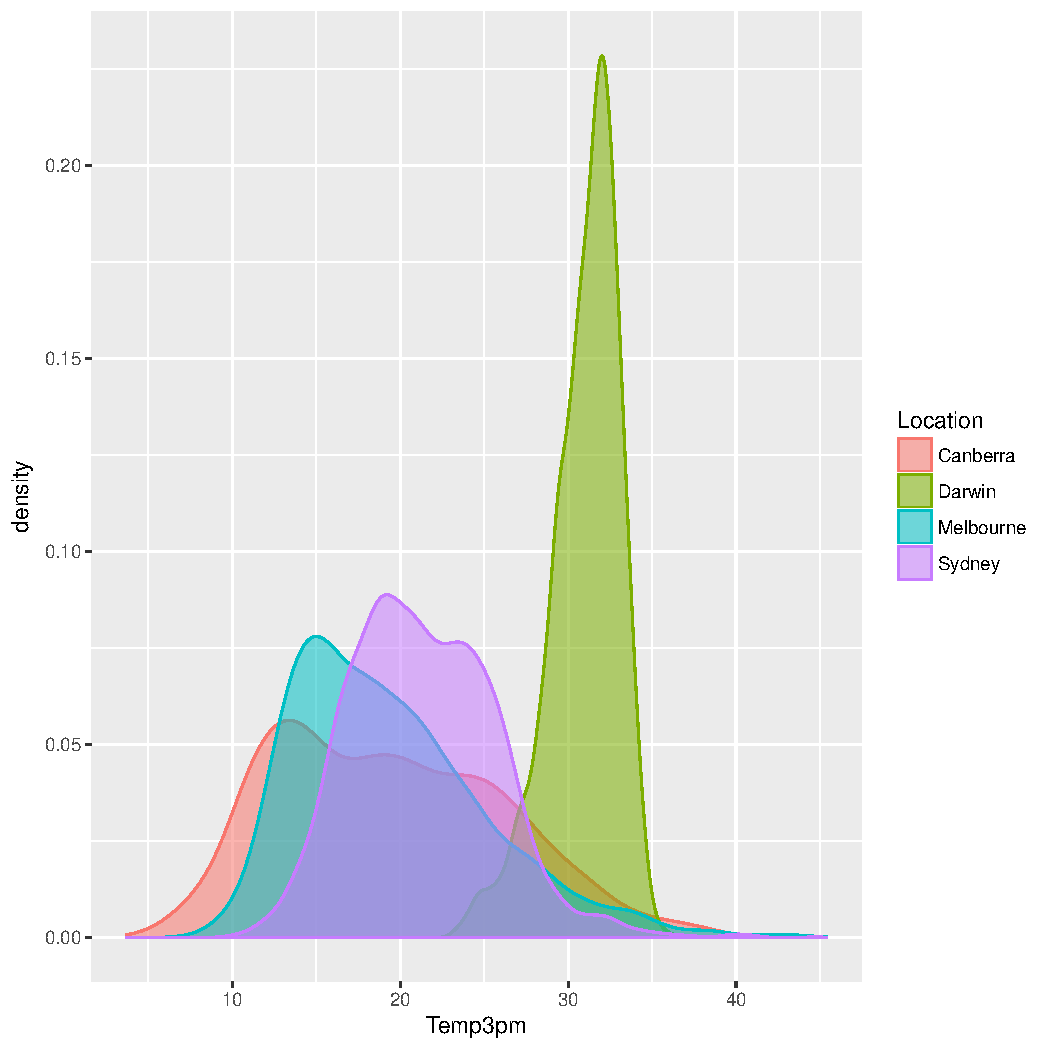
\includegraphics[width=\maxwidth]{figure/figure-1} 

\end{knitrout}



\end{document}
